% GNUPLOT: LaTeX picture with Postscript
\begingroup
  \makeatletter
  \providecommand\color[2][]{%
    \GenericError{(gnuplot) \space\space\space\@spaces}{%
      Package color not loaded in conjunction with
      terminal option `colourtext'%
    }{See the gnuplot documentation for explanation.%
    }{Either use 'blacktext' in gnuplot or load the package
      color.sty in LaTeX.}%
    \renewcommand\color[2][]{}%
  }%
  \providecommand\includegraphics[2][]{%
    \GenericError{(gnuplot) \space\space\space\@spaces}{%
      Package graphicx or graphics not loaded%
    }{See the gnuplot documentation for explanation.%
    }{The gnuplot epslatex terminal needs graphicx.sty or graphics.sty.}%
    \renewcommand\includegraphics[2][]{}%
  }%
  \providecommand\rotatebox[2]{#2}%
  \@ifundefined{ifGPcolor}{%
    \newif\ifGPcolor
    \GPcolortrue
  }{}%
  \@ifundefined{ifGPblacktext}{%
    \newif\ifGPblacktext
    \GPblacktexttrue
  }{}%
  % define a \g@addto@macro without @ in the name:
  \let\gplgaddtomacro\g@addto@macro
  % define empty templates for all commands taking text:
  \gdef\gplbacktext{}%
  \gdef\gplfronttext{}%
  \makeatother
  \ifGPblacktext
    % no textcolor at all
    \def\colorrgb#1{}%
    \def\colorgray#1{}%
  \else
    % gray or color?
    \ifGPcolor
      \def\colorrgb#1{\color[rgb]{#1}}%
      \def\colorgray#1{\color[gray]{#1}}%
      \expandafter\def\csname LTw\endcsname{\color{white}}%
      \expandafter\def\csname LTb\endcsname{\color{black}}%
      \expandafter\def\csname LTa\endcsname{\color{black}}%
      \expandafter\def\csname LT0\endcsname{\color[rgb]{1,0,0}}%
      \expandafter\def\csname LT1\endcsname{\color[rgb]{0,1,0}}%
      \expandafter\def\csname LT2\endcsname{\color[rgb]{0,0,1}}%
      \expandafter\def\csname LT3\endcsname{\color[rgb]{1,0,1}}%
      \expandafter\def\csname LT4\endcsname{\color[rgb]{0,1,1}}%
      \expandafter\def\csname LT5\endcsname{\color[rgb]{1,1,0}}%
      \expandafter\def\csname LT6\endcsname{\color[rgb]{0,0,0}}%
      \expandafter\def\csname LT7\endcsname{\color[rgb]{1,0.3,0}}%
      \expandafter\def\csname LT8\endcsname{\color[rgb]{0.5,0.5,0.5}}%
    \else
      % gray
      \def\colorrgb#1{\color{black}}%
      \def\colorgray#1{\color[gray]{#1}}%
      \expandafter\def\csname LTw\endcsname{\color{white}}%
      \expandafter\def\csname LTb\endcsname{\color{black}}%
      \expandafter\def\csname LTa\endcsname{\color{black}}%
      \expandafter\def\csname LT0\endcsname{\color{black}}%
      \expandafter\def\csname LT1\endcsname{\color{black}}%
      \expandafter\def\csname LT2\endcsname{\color{black}}%
      \expandafter\def\csname LT3\endcsname{\color{black}}%
      \expandafter\def\csname LT4\endcsname{\color{black}}%
      \expandafter\def\csname LT5\endcsname{\color{black}}%
      \expandafter\def\csname LT6\endcsname{\color{black}}%
      \expandafter\def\csname LT7\endcsname{\color{black}}%
      \expandafter\def\csname LT8\endcsname{\color{black}}%
    \fi
  \fi
    \setlength{\unitlength}{0.0500bp}%
    \ifx\gptboxheight\undefined%
      \newlength{\gptboxheight}%
      \newlength{\gptboxwidth}%
      \newsavebox{\gptboxtext}%
    \fi%
    \setlength{\fboxrule}{0.5pt}%
    \setlength{\fboxsep}{1pt}%
\begin{picture}(9620.00,9620.00)%
    \gplgaddtomacro\gplbacktext{%
      \csname LTb\endcsname%
      \put(779,5057){\makebox(0,0)[r]{\strut{}$0$}}%
      \csname LTb\endcsname%
      \put(779,5522){\makebox(0,0)[r]{\strut{}$500$}}%
      \csname LTb\endcsname%
      \put(779,5986){\makebox(0,0)[r]{\strut{}$1000$}}%
      \csname LTb\endcsname%
      \put(779,6451){\makebox(0,0)[r]{\strut{}$1500$}}%
      \csname LTb\endcsname%
      \put(779,6916){\makebox(0,0)[r]{\strut{}$2000$}}%
      \csname LTb\endcsname%
      \put(779,7381){\makebox(0,0)[r]{\strut{}$2500$}}%
      \csname LTb\endcsname%
      \put(779,7845){\makebox(0,0)[r]{\strut{}$3000$}}%
      \csname LTb\endcsname%
      \put(779,8310){\makebox(0,0)[r]{\strut{}$3500$}}%
      \csname LTb\endcsname%
      \put(779,8775){\makebox(0,0)[r]{\strut{}$4000$}}%
      \csname LTb\endcsname%
      \put(867,4858){\makebox(0,0){\strut{}$0$}}%
      \csname LTb\endcsname%
      \put(1509,4858){\makebox(0,0){\strut{}$200$}}%
      \csname LTb\endcsname%
      \put(2150,4858){\makebox(0,0){\strut{}$400$}}%
      \csname LTb\endcsname%
      \put(2792,4858){\makebox(0,0){\strut{}$600$}}%
      \csname LTb\endcsname%
      \put(3433,4858){\makebox(0,0){\strut{}$800$}}%
      \csname LTb\endcsname%
      \put(4075,4858){\makebox(0,0){\strut{}$1000$}}%
      \csname LTb\endcsname%
      \put(4163,5057){\makebox(0,0)[l]{\strut{} }}%
      \csname LTb\endcsname%
      \put(4163,5522){\makebox(0,0)[l]{\strut{} }}%
      \csname LTb\endcsname%
      \put(4163,5986){\makebox(0,0)[l]{\strut{} }}%
      \csname LTb\endcsname%
      \put(4163,6451){\makebox(0,0)[l]{\strut{} }}%
      \csname LTb\endcsname%
      \put(4163,6916){\makebox(0,0)[l]{\strut{} }}%
      \csname LTb\endcsname%
      \put(4163,7381){\makebox(0,0)[l]{\strut{} }}%
      \csname LTb\endcsname%
      \put(4163,7845){\makebox(0,0)[l]{\strut{} }}%
      \csname LTb\endcsname%
      \put(4163,8310){\makebox(0,0)[l]{\strut{} }}%
      \csname LTb\endcsname%
      \put(4163,8775){\makebox(0,0)[l]{\strut{} }}%
      \csname LTb\endcsname%
      \put(867,8974){\makebox(0,0){\strut{} }}%
      \csname LTb\endcsname%
      \put(1509,8974){\makebox(0,0){\strut{} }}%
      \csname LTb\endcsname%
      \put(2150,8974){\makebox(0,0){\strut{} }}%
      \csname LTb\endcsname%
      \put(2792,8974){\makebox(0,0){\strut{} }}%
      \csname LTb\endcsname%
      \put(3433,8974){\makebox(0,0){\strut{} }}%
      \csname LTb\endcsname%
      \put(4075,8974){\makebox(0,0){\strut{} }}%
    }%
    \gplgaddtomacro\gplfronttext{%
      \csname LTb\endcsname%
      \put(239,6916){\rotatebox{-270}{\makebox(0,0){\strut{}Time [s]}}}%
      \csname LTb\endcsname%
      \put(8827,8675){\makebox(0,0)[r]{\strut{}Picard unknown MGLevels2}}%
      \csname LTb\endcsname%
      \put(8827,8476){\makebox(0,0)[r]{\strut{}Picard SoftGMRES Swz w Coarse MGLevels2}}%
      \csname LTb\endcsname%
      \put(8827,8277){\makebox(0,0)[r]{\strut{}NewtonGmres Swz w Coarse Overlap MGLevels2}}%
      \csname LTb\endcsname%
      \put(8827,8078){\makebox(0,0)[r]{\strut{}NewtonGmres Swz Kcycle w Coarse Overlap MGLevels2}}%
    }%
    \gplgaddtomacro\gplbacktext{%
      \csname LTb\endcsname%
      \put(691,684){\makebox(0,0)[r]{\strut{}$0$}}%
      \csname LTb\endcsname%
      \put(691,1238){\makebox(0,0)[r]{\strut{}$20$}}%
      \csname LTb\endcsname%
      \put(691,1792){\makebox(0,0)[r]{\strut{}$40$}}%
      \csname LTb\endcsname%
      \put(691,2346){\makebox(0,0)[r]{\strut{}$60$}}%
      \csname LTb\endcsname%
      \put(691,2900){\makebox(0,0)[r]{\strut{}$80$}}%
      \csname LTb\endcsname%
      \put(691,3454){\makebox(0,0)[r]{\strut{}$100$}}%
      \csname LTb\endcsname%
      \put(691,4008){\makebox(0,0)[r]{\strut{}$120$}}%
      \csname LTb\endcsname%
      \put(691,4562){\makebox(0,0)[r]{\strut{}$140$}}%
      \csname LTb\endcsname%
      \put(779,485){\makebox(0,0){\strut{}$0$}}%
      \csname LTb\endcsname%
      \put(1438,485){\makebox(0,0){\strut{}$1000$}}%
      \csname LTb\endcsname%
      \put(2097,485){\makebox(0,0){\strut{}$2000$}}%
      \csname LTb\endcsname%
      \put(2757,485){\makebox(0,0){\strut{}$3000$}}%
      \csname LTb\endcsname%
      \put(3416,485){\makebox(0,0){\strut{}$4000$}}%
      \csname LTb\endcsname%
      \put(4075,485){\makebox(0,0){\strut{}$5000$}}%
      \csname LTb\endcsname%
      \put(4163,684){\makebox(0,0)[l]{\strut{} }}%
      \csname LTb\endcsname%
      \put(4163,1238){\makebox(0,0)[l]{\strut{} }}%
      \csname LTb\endcsname%
      \put(4163,1792){\makebox(0,0)[l]{\strut{} }}%
      \csname LTb\endcsname%
      \put(4163,2346){\makebox(0,0)[l]{\strut{} }}%
      \csname LTb\endcsname%
      \put(4163,2900){\makebox(0,0)[l]{\strut{} }}%
      \csname LTb\endcsname%
      \put(4163,3454){\makebox(0,0)[l]{\strut{} }}%
      \csname LTb\endcsname%
      \put(4163,4008){\makebox(0,0)[l]{\strut{} }}%
      \csname LTb\endcsname%
      \put(4163,4562){\makebox(0,0)[l]{\strut{} }}%
      \csname LTb\endcsname%
      \put(779,4761){\makebox(0,0){\strut{} }}%
      \csname LTb\endcsname%
      \put(1438,4761){\makebox(0,0){\strut{} }}%
      \csname LTb\endcsname%
      \put(2097,4761){\makebox(0,0){\strut{} }}%
      \csname LTb\endcsname%
      \put(2757,4761){\makebox(0,0){\strut{} }}%
      \csname LTb\endcsname%
      \put(3416,4761){\makebox(0,0){\strut{} }}%
      \csname LTb\endcsname%
      \put(4075,4761){\makebox(0,0){\strut{} }}%
    }%
    \gplgaddtomacro\gplfronttext{%
      \csname LTb\endcsname%
      \put(239,2623){\rotatebox{-270}{\makebox(0,0){\strut{}Speedup}}}%
      \csname LTb\endcsname%
      \put(2427,187){\makebox(0,0){\strut{}Grid:NoOfCells}}%
      \csname LTb\endcsname%
      \put(8827,4462){\makebox(0,0)[r]{\strut{}Picard unknown MGLevels2}}%
      \csname LTb\endcsname%
      \put(8827,4263){\makebox(0,0)[r]{\strut{}Picard SoftGMRES Swz w Coarse MGLevels2}}%
      \csname LTb\endcsname%
      \put(8827,4064){\makebox(0,0)[r]{\strut{}NewtonGmres Swz w Coarse Overlap MGLevels2}}%
      \csname LTb\endcsname%
      \put(8827,3865){\makebox(0,0)[r]{\strut{}NewtonGmres Swz Kcycle w Coarse Overlap MGLevels2}}%
      \csname LTb\endcsname%
      \put(8827,3666){\makebox(0,0)[r]{\strut{}Ideal}}%
    }%
    \gplbacktext
    \put(0,0){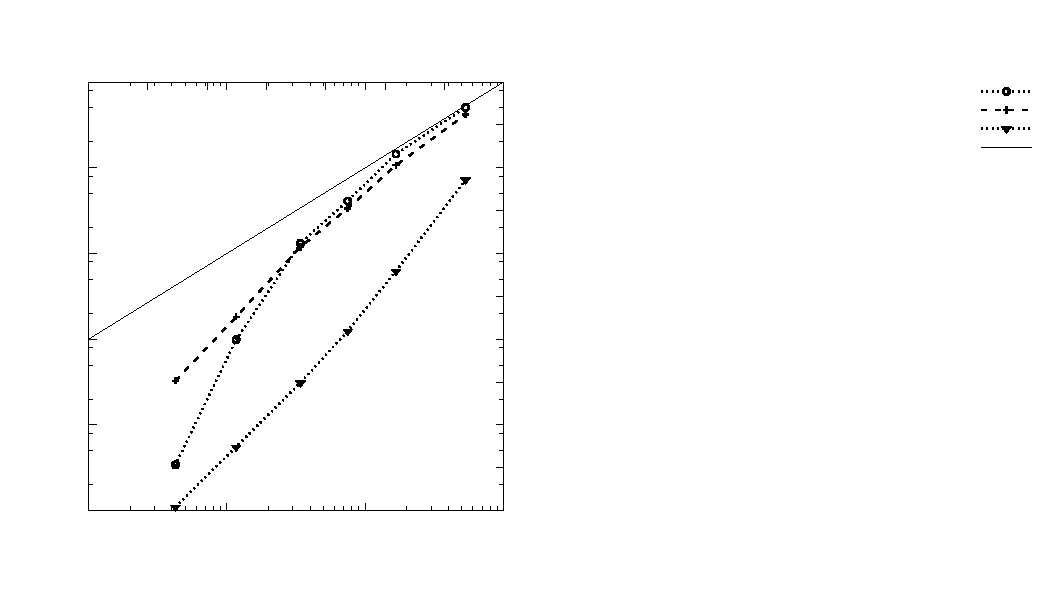
\includegraphics{NodePerformance}}%
    \gplfronttext
  \end{picture}%
\endgroup
